% vim:set et sw=2 ts=4 tw=72:
\chapter{Discussion}\label{cha:discussion}

This chapter provides further discussion on the results and observations
from the study evaluating \tool{}. Included are observations that could
lead to improvements in the current DAG visualizations, the comments
from a release manager, and work toward applying the \mt{} model and
visualizations to other repositories.

\section{Interpreting the Results}\label{sec:interpreting_the_results}

Overall, the results indicate that \tool{} is able to improve the
correctness and accuracy of responses to various summarization tasks,
and decrease the time taken to produce the results. This doesn't come as
a surprise since the goal of the \mt{} model and the visualizations in
\tool{} are to provide better conceptual understanding and
summarizations of merges, while Gitk and DAG visualizations are designed
to show the topology of the entire repository. Since there are no other
tools for showing how a commit is integrated, and the topology of the
DAG does contain this information, the DAG visualization is used as a
proxy to show how a commit reaches the master branch.

One area of interest is the comparison of \tool{} and Gitk on
correctness in task T10, determining the modules modified in a merge.
Again, modules are no inherent to Git and are a property of the commits
in the Linux repository, the module is found in the summary of the
commit logs. In this task, there was not a statistically significant
difference in the number of correct responses between \tool{} and Gitk,
and, while significant, the effect on accuracy was also small. This is
interesting because \tool{} provided this information directly, while
users would have to look at the commit logs to determine this
information from Gitk. Further inspection of the merges show that this
was the only task where the correct answer was in the commit that was
provided, and actually required no aggregation of the results.

Another area of interest are the time results for task T7. This is the
only task where merge size had a significant impact on the performance
of the participants. There was not a statistically significant
difference in the time taken to respond to this task between the two
tools; however, the effect size indicates that the tool has a medium
effect on the time taken to respond. This is likely due to the sample
size. In the other tasks, the responses 11 responses for both merges
were combined, effectively doubling this number, creating 22 samples.
Since there was a difference in the time taken to respond given the
merge size, the results had to be analyzed separately. 11 samples is
quite small, and is likely not enough to have a 95\% confidence in the
results.

\section{Study Observations}\label{sec:study_observations}

Identifying the master branch was an issue that consistently came up
among all participants during the study. Some participants assumed that
the first line in the DAG visualization indicated the master branch,
while others assumed that the next branch tag indicated the master
branch. The DAG visualization provides no indication of which branch is
the master branch. Furthermore, the visualization in Gitk is not
consistent, branch colors and positions change between runs; identifying
the branch once does not guarantee that it is identifiable after
restarting Gitk.

If the participants were able to easily identify the master branch, the
results from the study would likely be very different. This would be
most prominent in the summarization portion of the small merge, since
summarizing a single item is trivial, but the issue was identifying that
there was only a single item, which is currently not trivial. With more
than 25\% of the merges into Linux being single-commit merges, it is
important that users are able to identify them and understand the
changes being made within them. The structure of a single-commit tree is
identical to the structure of a flat tree, all commits are merged
directly into the master branch, passing through no other merges on the
way. Flat trees are the most common form of tree in the kernel
repository. To improve the visualization of the DAG for providing an
effective visualization for summarization and comprehension of flat
trees, it would likely be sufficient to indicate the master branch.
For the non-flat trees, a more powerful structure would likely be
necessary.

\section{Comments From a Release Manager}\label{sec:comments_from_a_release_manager}

One of the participants in the study had worked as a release manager for
more than three years, working with both SVN and CVS repositories. The
goal of a release manager is to determine how to merge the branches of a
repository in such a way that it minimizes merge conflicts and maintains
the meaning of the underlying source code. This section contains
insights from this participant, providing comments on ways that could
improve \tool{} and the \mt{} model.

Contributors making merges need to understand more than just what merges
a commit was collected into before reaching the repository of the
contributor. It is also important to understand order that the related
commits were made, as the order tells the story of what the developer
was thinking as they were writing the changes. The visualization of the
\mt{} in \tool{} does not order the commits, randomly ordering them in
each level as atomic units.

This is the primary reason behind why this participant would ask to use
both tools simultaneously. \tool{} is able to help with the aggregation
of the information, and provide a better understanding of the next merge
involved in integrating this commit, but the DAG visualization in Gitk
provides the full story of the commit instead of hiding it behind a
layer of abstraction.

The comments from this participant were very insightful, and will help
to improve the \mt{} model.

\section{Generalization}\label{sec:generalization}

The purpose of generalizing the algorithm is two-fold. First, providing
a means of working with more than one repository in an efficient manner.
Second, adjusting the model to take into account the comments made, so
that it captures the order of the commits, and thus, the story behind
how an author was working.

Due to the requirements needed to construct the model, it is likely that
it won't be possible to create accurate \mt{s} for most repositories.
First, it must be possible to identify the master branch, which can be
confounded by \foxtrot{} merges. It was due to the strict merge
discipline found in the Linux repository that made this work possible.
Second, the repository must make use of merge commits, fast-forward
merges will hide the existence of a merge. Assuming that \foxtrot{}
merges do not confound the master branch, and that the repository makes
use of merge commits, it is possible to create the \mt{s} of the
repository.

The updated model takes the \mt{} from before, and overlays it back on
the DAG; the new model still shows the path that a commit took to reach
the master branch, but removes branch links. Only commits made
immediately after the branch are leaves.

Going back to the example in Chapter~\ref{chap:Model}, the DAG of the
example events repeated in Figure~\ref{fig:example_DAG_again}, and the
original \mt{} repeated in Figure~\ref{fig:example_MT_again}. In this
model, it appears that the code in 3 is merged at 5, and there is no
notion of what interaction it has with the commits that are in that
branch. The new model should change the story, showing that 5 merges the
changes made in 3 into the changes made in 2. 4 will still be ignored as
it is already in the master branch. Then 7 modifies the changes that are
at 5. From there, 9 takes the changes made in 8 and 6, and merges them
into 7. This new model should maintain the base branch of the merge, in
the case of 9, it is the yellow branch. The new model is shown in
Figure~\ref{fig:repoDAGTree}.

\begin{figure}[htbp]
  \centering
  \resizebox{0.8\textwidth}{!}{
  \begin{tikzpicture}[auto, on grid, semithick, state/.style={circle, text=black, black}]
    \node[state, black] (1) {1};
    \node[state, black, above right= of 1] (2) {2};
    \node[state, black, above right= 2cm and 1cm of 2] (3) {3};
    \node[state, black, right= 2cm of 1] (4) {4};
    \node[state, black, above right=of 4] (5) {5};
    \node[state, black, above right=of 5] (6) {6};
    \node[state, black, right=of 5] (7) {7};
    \node[state, black, above right= 2cm and 1cm of 7](8) {8};
    \node[state, black, right= 2cm of 7] (9) {9};
    \node[state, black, right=of 9] (10) {10};
    \node[state, black, below right=of 9] (11) {11};
    \node[state, black, draw=chartblue, below right=of 10] (12) {12};

    \draw (12) edge[-stealth] (11) edge[-stealth] (10);
    \draw (11) edge[-stealth] (4) edge[-stealth] (9);
    \draw (10) edge[-stealth] (9);
    \draw (9) edge[-stealth] (8) edge[-stealth] (6)
              edge[-stealth] (7);
    \draw (8) edge[-stealth] (7);
    \draw (7) edge[-stealth] (5);
    \draw (6) edge[-stealth] (5);
    \draw (5) edge[-stealth] (3) edge[-stealth] (2)
              edge[-stealth] (4);
    \draw (4) edge[-stealth] (1);
    \draw (3) edge[-stealth] (2);
    \draw (2) edge[-stealth] (1);
  \end{tikzpicture}
  }
  \caption{The DAG of the repository events}
  \label{fig:example_DAG_again}
%\vspace{-3mm}
\end{figure}

\begin{figure}[htpb]
  \centering
  \resizebox{0.8\textwidth}{!}{
    \begin{tikzpicture}[auto, on grid, semithick, node distance=1cm, state/.style={circle, text=black, minimum size=7mm}]

      \node[state, draw=chartblue] (1) {1};
      \node[state, draw=chartblue, right=of 1] (4) {4};
      \node[state, draw=chartblue, right=of 4] (11) {11};
      \node[state, draw=chartblue, right=2.5cm of 11] (12) {12};

      \node[state, draw=chartyellow, above right= 1cm and 0.5cm of 11] (7) {7};
      \node[state, draw=chartyellow, above left= 1cm and 0.5cm of 11] (5) {5};
      \node[state, draw=chartyellow, right=of 7] (9) {9};
      \node[state, draw=chartyellow, left=of 5] (2) {2};
      \node[state, draw=chartmagenta, above=of 5] (3) {3};
      \node[state, draw=chartmagenta, above left=1cm and 0.5cm of 9] (6) {6};
      \node[state, draw=chartmagenta, above right=1cm and 0.5cm of 9] (8){8};
      \node[state, draw=chartyellow, above=of 12] (10) {10};

      \draw (11) edge[chartyellow, stealth-] (2) edge[chartyellow, stealth-] (5) edge[chartyellow, stealth-] (7) edge[chartyellow, stealth-] (9)
      (5) edge[chartmagenta, stealth-] (3)
      (9) edge[chartmagenta, stealth-] (6) edge[chartmagenta, stealth-] (8)
      (12) edge[chartyellow, stealth-] (10);
    \end{tikzpicture}
  }
  \caption{The original \mt{} built from the DAG in Figure~\ref{fig:example_DAG_again}}
  \label{fig:example_MT_again}
\end{figure}


\begin{figure}[htbp]
  \centering
  \resizebox{0.8\textwidth}{!}{
  \begin{tikzpicture}[auto, on grid, semithick, state/.style={circle, text=black}]

    \draw[chartblue]
      (-0.5, -0.5) -- (8.5, -0.5) -- (8.5, 0.5) -- (-0.5, 0.5) -- (-0.5, -0.5);

    \node[state, draw=chartblue] (1) {1};
    \node[state, draw=chartyellow, above right= of 1] (2) {2};
    \node[state, draw=chartmagenta, above right= 2cm and 1cm of 2] (3) {3};
    \node[state, draw=chartblue, right= 2cm of 1] (4) {4};
    \node[state, draw=chartyellow, above right=of 4] (5) {5};
    \node[state, draw=chartred, above right=of 5] (6) {6};
    \node[state, draw=chartyellow, right=of 5] (7) {7};
    \node[state, draw=chartmagenta, above right= 2cm and 1cm of 7](8) {8};
    \node[state, draw=chartyellow, right= 2cm of 7] (9) {9};
    \node[state, draw=chartyellow, right=of 9] (10) {10};
    \node[state, draw=chartblue, below right=of 9] (11) {11};
    \node[state, draw=chartblue, below right=of 10] (12) {12};

    \draw (2) edge[chartyellow, -stealth] (5)
          (3) edge[chartmagenta, -stealth](5)
          (5) edge[chartyellow, -stealth] (7)
          (7) edge[chartyellow, -stealth] (9)
          (6) edge[chartred, -stealth] (9)
          (8) edge[chartmagenta, -stealth] (9)
          (9) edge[chartyellow, -stealth] (11)
          (10) edge[chartyellow, -stealth] (12);
  \end{tikzpicture}
  }
  \caption{The \mt{} overlayed on the inverted DAG to show the order
    that commits are created, as ell as the merge sequence for the DAG
    in Figure~\ref{fig:example_DAG_again}. This requires a
    post-processing step to combine the \mt produced by
    Algorithm~\ref{fig:alg} and the DAG.}
\label{fig:repoDAGTree}
\vspace{-3mm}
\end{figure}

The second goal behind the changes is to make it more accessible to
other repositories. To do this, I designed a small webpage that would
interact with public Bitbucket repositories and generate \mt{s} from the
DAGs of those repositories, shown in Figure~\ref{fig:bitbucket_plugin}.
Since the contents of the repository are accessed through a public API,
it is important to consider bandwidth usage and limit the amount of data
being consumed. Building a single \mt{} does not require information for
every repository event in the repository, only the subset of repository
events that will be present in the \mt{}. Algorithm~\ref{fig:alg}
requires information for the entire repository, and constructs every
\mt{} simultaneously. I designed a second algorithm that constructs only
a single \mt{}, and attempts to use a subset of the repository events in
the repository to do this. The new algorithm is broken into two phases.

The first phase performs three operations; first, it tracks the master
branch of the repository; second, it labels each repository event with
the depth, or the number of merges that a given node will have to pass
through to reach the master branch; third, inverting and pruning the
DAG\@. The first phase takes a repository event along the master branch
as input, and returns a pruned and inverted DAG with the nodes annotated
with the depths. The first phase is shown in
Algorithm~\ref{alg:generalized_phase_I}. The second phase is designed to
resolve the \mt{} from the inverted DAG\@. The second phase is shown in
Algorithm~\ref{alg:generalized_phase_II}.

\begin{figure}[htpb]
  \centering
  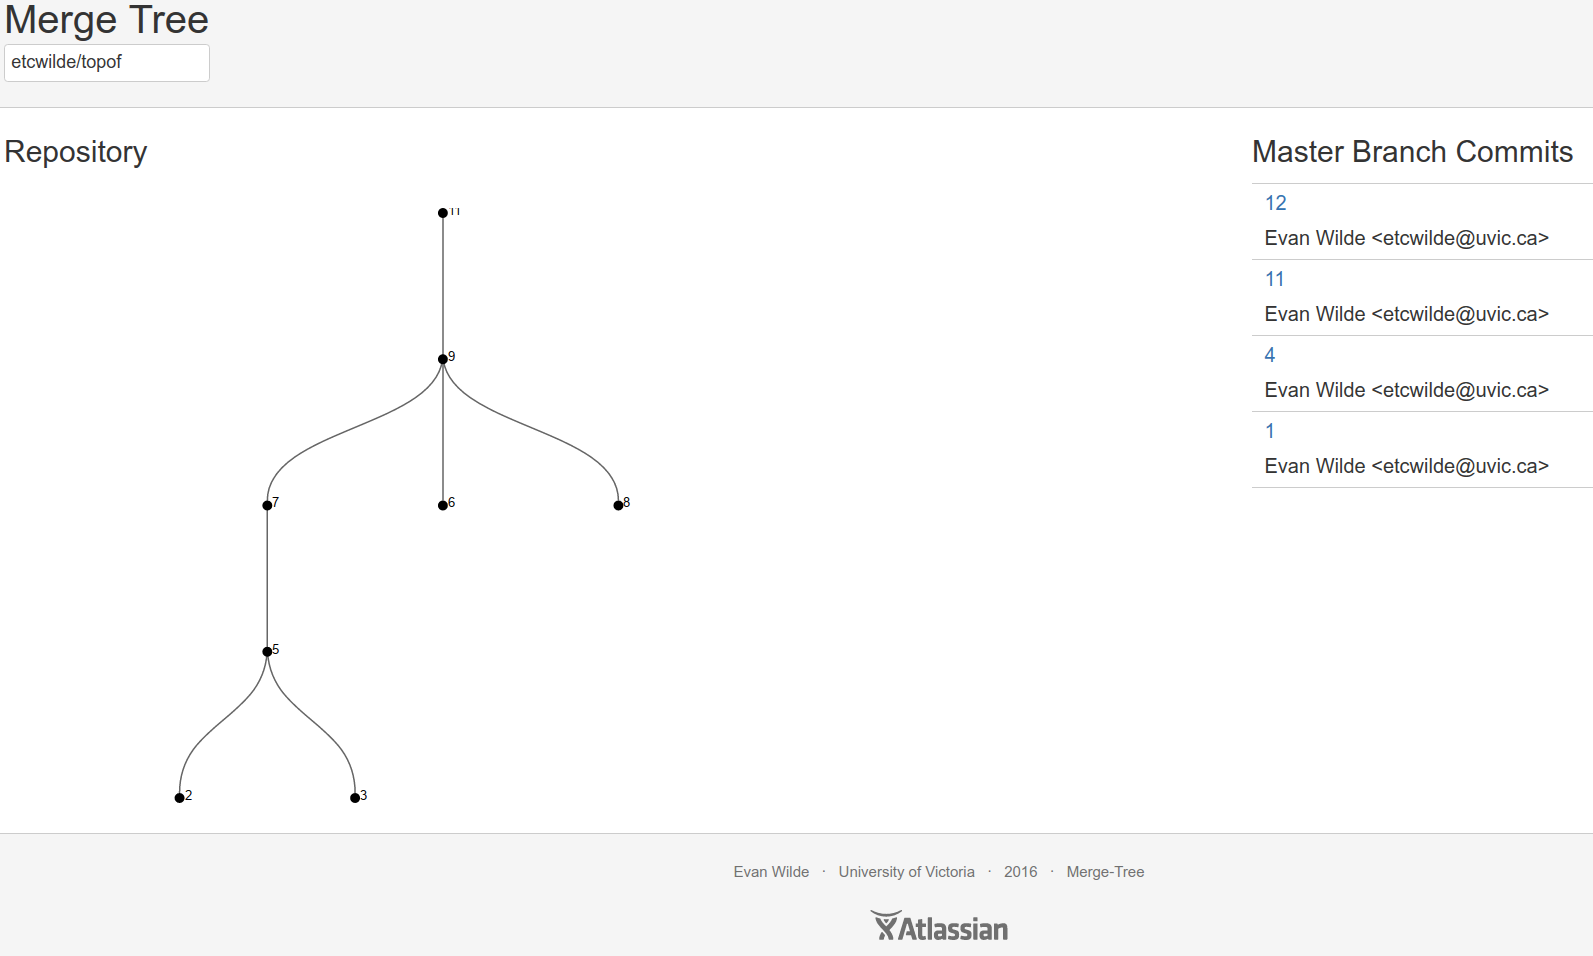
\includegraphics[width=0.8\linewidth]{Figures/bitbucket_plugin.png}
  \caption{Bitbucket plugin showing the updated \mt{} on the repository
  DAG in Figure~\ref{fig:example_DAG_again}.}
  \label{fig:bitbucket_plugin}
\end{figure}

\begin{algorithm}
  \caption{Computing the generalized Merge Tree: Phase 1}
  \label{alg:generalized_phase_I}
  \begin{algorithmic}[1]
    \Function{Phase 1}{initial commit $root$} : updated tree
    \State $openBranches \gets 0$
    \State $Q \gets root$
    \Do
    \State $cur \gets Q.dequeue$
    \State $parents \gets cur.parents$
    \State $openBranches \gets openBranches + parents.length - 1$
    \For{$index, parent \in parents$}
    \If{$parent.depth$ is $undefined$}
    \State $parent.depth \gets cur.depth + index$
    \ElsIf {$cur.depth > parent.depth$}
    \State $openBranches \gets openBranches - 1$
    \ElsIf {$cur.depth < parent.depth$}
    \State $openBranches \gets openBranches - 1$
    \State $parent.depth \gets cur.depth$
    \EndIf
    \State $parent.children \gets cur$
    \If{$parent$ has not been visited}
    \State $Q \gets parent$
    \State $parent.visited \gets True$
    \EndIf
    \EndFor
    \doWhile{$Q$ not empty and $openBranches \ne 0$ }
    \EndFunction
  \end{algorithmic}
\end{algorithm}

Unlike the original algorithm, this algorithm works as a breadth-first
traversal of the DAG. Starting at the root node, the algorithm collects
the parents of the node. If the root node is not a merge, but a commit
made directly in the master branch, the \mt{} of this node will only
contain this node. The node will have only parent, which is the next
event on the master branch toward the initial commit. This parent will
get pushed onto the processing Queue, but the number of open branches
will remain zero, since the root was a commit, and introduced no new
branches that would then need to reach a branching point. Since the
number of open branches is still zero, the algorithm terminates without
further traversal. If the node is a merge node, it will introduce $p -
1$ new branches that it is merging, where $p$ is the number of parents.
This number is $p - 1$ because the first parent is on the same branch as
the current node, and the current branch is already open. Each of the
$p-1$ branches need to reach a branch point before the algorithm can
terminate. This does not handle the case where a branch could contain a
dangling Initial commit, where a branch with an unrelated history is
merged into the repository. This is usually found in situations where a
separate repository is merged into the current repository, and did the
separate repository was not a clone or a fork of the current repository.
The Linux repository has 3 dangling initial commits and 1 normal initial
commit, which are found with the command
\verb|git rev-list --max-parents=0 HEAD|.

The sequence of \verb|if| statements from line 9 to line 16 of the
algorithm are used for resolving the type of branch and the node depth.
If the parent has not yet been assigned a depth, then the parent has not
been visited yet. We assume that it is at the same depth as the current
node plus, the index. The first parent is on the same branch, the index
is 0, so the depth of the parent will be the same as the current node.
Subsequent parents will be assigned accordingly. This assignment of
depths retains more information that the original \mt{} stricture, since
the depth includes the order that the branches were merged. If the
parent has a depth associated with it there are three possibilities for
this depth, the depths could be equal, the depth of the parent could be
less than the depth of the current node, or the depth of the parent
could be greater than the depth of the current node. If both nodes are
at the same depth no actions need to take place, both nodes are on the
same branch, so no branch points are detected. In the second case, when
the depth of the current node is greater than the depth of the parent,
this indicates that the parent is the branch node for the current node,
the number of open branches is decremented to indicate this. If the
depth of the current node is less than the depth of the parent, this is
also a branch point, but it indicates that the depth of the parent was
incorrectly assigned. This situation can occur when a branch point has
fewer repository events on the side branch than on the main branch, as
seen in Figure~\ref{fig:graph_1}. In this situation, the traversal
starts at $F$ where the open branches increases by one to include the
green branch. Following the breadth-first approach, $E$ will be assigned
the same depth as $F$, while $C$ will be assigned a depth of $F + 1$. On
the next iteration, $D$ will be assigned the same depth as $F$ and $A$
will be assigned the depth of $C$, when it should have the same depth as
$F$. In this situation, $B$ will detect that $A$ as a depth that is
larger than the correct depth. The green branch did not detect that the
branch closed at $A$ since the depth of $A$ was undefined, so $B$ must
replace the depth of $A$ with the depth of $B$, which is the same as the
depth of $F$, and decrement the number of open branches since the green
branch did not detect this. In these situations, more nodes will be
imported than the nodes required, if $A$ were not the initial commit.
Once a depth has been assigned to the parent, the parent is added to the
processing queue if it has not already been visited.

\begin{figure}[htpb]
  \centering
  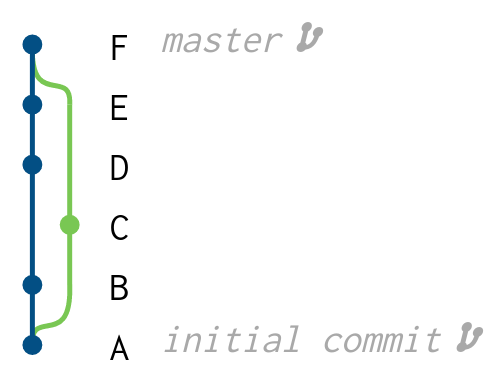
\includegraphics[height=4cm]{Figures/graph_1.png}
  \caption{Situation where an incorrect depth will be assigned to node
    $A$ initially before being resolved by $B$}
  \label{fig:graph_1}
\end{figure}

\begin{table}[htpb]
  \centering
  \caption{Example traversal of the example DAG in
    Figure~\ref{fig:example_DAG_again} starting at merge 11.}
  \label{tab:ex_traversal}
  \begin{tabular}{cccc|rl}
    \toprule
    Current & Parents & Open Branches & Q       & Visited : Depth & Children\\\midrule
    -       & -       & 0             & 11      & 11      : 0     & \\
    11      & 4,9     & 1             & 4,9     & 4       : 0     & 11, 5\\
    4       & 1       & 1             & 9,1     & 9       : 1     & 11\\
    9       & 7,6,8   & 3             & 1,7,6,8 & 1       : 0     & 4\\
    1       &         & 3             & 7,6,8   & 7       : 1     & 9, 8\\
    7       & 5       & 3             & 6,8,5   & 6       : 2     & 9\\
    6       & 5       & 2             & 8,5     & 8       : 3     & 9\\
    8       & 7       & 1             & 5       & 5       : 1     & 7, 6\\
    5       & 4,2,3   & 2             & 2,3     & 2       : 1     & 5, 3\\
    2       & 1       & 1             & 3       & 3       : 2     & 5\\
    3       & 2       & 0             &         &                 & \\
    \bottomrule
  \end{tabular}
\end{table}

Table~\ref{tab:ex_traversal}, shows the steps in the traversal of the
DAG in Figure~\ref{fig:example_DAG_again}, starting at merge 11. Current
indicates the node being visited at $cur$, Parents, the $parents$ of
$cur$. Open Branches indicates the number of open branches, stored in
$openBranches$. Q are the nodes in the processing queue. Visited and
depth are stored together in this table, simply showing which nodes have
been visited and the depth of those nodes. Visited is not in perfect
order with the steps to the left of the vertical bar, but is kept as a
ledger. Children indicates the children in the reversed DAG of the node
name in Visited. The Children in the table become the candidate parents
of each node, when resolving the trees.

Continuing with the example; open branches is initialized to 0, and the
root, 11 is pushed onto the work queue. Since 11 is provided as the
root, we assume that it has a depth of 0, and we add it to the visited
list.

11 is dequeued from the work queue, and the parents 4 and 9 are resolved
from the DAG. Open branches is updated to 1. Working through the
parents, neither parent have an assigned depth, so the parent depths are
assigned. 4 is in the first position, so it is on the same branch depth
as 11, and 9 is in the second position, so it is one higher than the
branch depth of 11. 11 is added to the children lists of 4 and 9, which
provides the inverted links of the DAG.

4 is dequeued from the work queue. 4 only has one parent, 1, so the
number of open branches remains 1. 1 has a depth of 0 since it is on the
same branch as 4. 4 is added as a child of 1, and finally 1 is pushed to
the processing queue and added to the visited list.

9 is dequeued from the work queue. 9 has three parents, 7, 6, and 8, so
the number of open branches advances to 3. 9 has a depth of 1 and none
of 7, 6, or 8 have a depth value assigned yet, so 7 is assigned a depth
of 1, 6 a depth of 2, and 8 a depth of 3. Each of these have 9 added to
the children list, and are pushed onto the work queue and the visited
list.

1 is dequeued from the work queue, and has no parents since it is the
initial commit of the repository. No work needs to be done on 1.

7 is dequeued from the work queue. 7 has one parent, 5. The number of
open branches remains the same. 5 does not have an associated depth
value assigned yet, and is the first parent of 7, so 5 is assigned a
depth of 1. 7 is added to the children list of 5, 5 is pushed to the
work queue and added to the list of visited nodes.

6 is dequeued from the work queue. 6 has one parent, 5. The number of
open branches remains the same for now. 5 already has an associated
depth of 1, and 6 has a depth of 2. Since the depth of the current node
is greater than the depth of the parent, it indicates that this branch
is closing, so the number of open branches is decremented to 2. 6 is
added to the children list of 5. Since 5 is already in the visited list,
it is not added again.

8 is dequeued from the work queue. 8 has one parent, 7. The number of
open branches remains the same for now. 7 already has an associated
depth of 1, and 8 has a depth of 3. Since the depth of 8 is greater than
the depth of 7, the number of open branches is decremented to 1. 8 is
added to the list of children of 7.

I can continue with the expansion of node 5, but I think that this is
sufficient for the understanding of phase 1.

\begin{algorithm}
  \caption{Computing the generalized Merge Tree: Phase 2}
  \label{alg:generalized_phase_II}
  \begin{algorithmic}[1]
    \Function{Phase 2}{initial commit $root$} : Merge tree
    \State $tree.root \gets root$
    \State $Q$ // Empty Queue

    \State $parents \gets root.parents$
    \State $parents \gets tail\ parents$
    \For {$parent \in parents$}
    \State $realParent \gets min(\forall child \in parent.children,\ parent.depth >= child.depth)$
    \If {$realParent$ is $root$}
    \State $root.children \gets parent$
    \State $parent.parent \gets root$
    \State $Q \gets parent$
    \EndIf
    \EndFor

    \While{$Q$ not empty}
    \State $cur \gets Q.dequeue$
    \State $parents \gets cur.parents$
    \For{$parent \in parents$}
    \State $realParent \gets min(\forall child \in parent.children,\ parent.depth >= child.depth)$
    \If {$realParent$ is $cur$}
    \State $cur.children \gets parent$
    \State $parent.parent \gets cur$
    \State $Q \gets parent$
    \EndIf

    \EndFor
    \EndWhile

    \EndFunction
  \end{algorithmic}
\end{algorithm}

Phase 2 takes the forward DAG, inverted DAG, and node depths to resolve
the actual \mt{}. Again, starting at the root merge into the master
branch, this phase uses a breadth-first approach to find the shortest
paths for a given commit to reach the master branch. Since this is the
phase where the parent-child relationship is flipped completely to form
the tree, the terminology becomes difficult to follow. The $parents$ are
the DAG parents, the $realparent$ is the tree parent, the $realParent$
is one of the children from the previous phase. The algorithm looks
through each of the DAG parents of the current node. A $realParent$ is
calculated for that parent from the children of the parent. The
$realParent$ is the DAG child that has the smallest depth that is still
greater than the depth of the parent. Essentially, it is looking for the
child that is on the branch closest to the branch, in terms of depth,
that the parent is on. If the $realParent$ is the current node, then the
current node is the tree parent to the parent. The DAG parent currently
being observed is added to the tree children of the current node, and
the DAG parent is added to the processing queue. \evan{If this makes any
  sense at all, I will be very happy!}

The algorithm has not yet been evaluated against the results of the
original algorithm, or on the accuracy in the context of the kernel.
Small repositories have been used to verify that it produces the correct
trees for various repository topologies. The set of small repositories
used test for many situations, but are not comprehensive. Further
evaluation on the quality of the \mt{s} produced is required before the
algorithm and the new model are ready for a full user study. The new
algorithm is not minimal, the subset of the DAG contains nodes that are
not required in the final tree. A more efficient algorithm may be
possible. Once the results of the algorithm have been fully assessed,
member checking may be a potential means of determining that the new
model and new algorithm satisfy the shortcomings of the original model.

\section{Threats to Validity}\label{sec:threats_to_validity}

While precautions were taken to mitigate threats to the validity, for
pragmatic reasons and other errors, some threats must be taken into
account when considering the results. These threats, the mitigation
techniques, and the steps to minimize other threats are provided in this
section.

\subsection{Internal Validity}\label{sub:internal_validity}

In order to minimize the effects of order bias, the order that the tools
were used, the commits were analyzed, and the tasks were performed was
randomized for each participant. This leaves a lot of room for error in
the part of the person performing the study. To minimize this room for
error, a script was used to generate the exact text that needed to be
used during the study. While this method proved to be very useful, I
omitted one task during the course on one study. As a result, the
information collected from this participant were removed from the pool
during analysis.

The merges chosen from the repository may not be a good representation
of the merges in the repository. These merges were chosen to be from the
first and second quartile to help select merges that were of common
sizes. Of course, these are two merges out of thousands, and were
selected randomly from the set of all merges.

The answers provided by participants to earlier tasks were not taken
into account when evaluating the correctness or accuracies to following
tasks. The results of an incorrect answer may impact the results of the
tasks that followed. If the participant was unable to determine the
correct commits that were being merged, then none of the summarizations
would be correct, even if the response was correct given the commits
they identified. A future study could mitigate this by providing the
correct set of commits that are being merged between the conceptual and
summarization task sets to limit the propagation of errors.

\subsection{External validity}\label{sub:external_validity}

While many online git resources, Gitk, and the git command line provide
visualizations of the DAG, many participants were unfamiliar with the
DAG visualizations. Other tools than Gitk and the command line may
provide better summarizations and different visualizations, I am not
aware of any. I investigated the use of other GUI tools on the git
website, but none were able to produce visualizations for repositories
that are at the size of the Linux kernel repository, except for Gitk and
the git command line. While this may have had an effect on the results,
the tools listed on the website provide a very similar visual DAG
metaphor to the visualization in Gitk.

The participants in the study were students, some with industrial
experience. Most participants had worked with relatively few
collaborators on academic projects. Many of the participants had worked
with larger repositories while performing a research study. Even though
the participants have worked with large repositories during the course
of their research, professional developers are the target audience of
this tool, so working with professional developers would provide more
meaningful results.

\section{Limitations}\label{sec:limitations}

The model is designed with the Linux repository in mind. The viability
of \mt{s} to provide useful and accurate information relies on a few
properties of the underlying repository. The repository must use a
branch and merge structure. Some repositories, like the OCaml
repository, commit directly into the master branch. At release time, a
branch is created for the version being released. Patches to the version
are added as necessary. The release branch is never merged back into the
master branch. Since \mt{s} are designed to show how a commit is
integrated into the master branch, an \mt{} will not help with a
repository with this structure.

Repositories cannot have foxtrots. A foxtrot confounds the master
branch, making it impossible to properly determine where the integrating
merge occurs. The algorithm will continue to process repositories
containing foxtrots; however, the resulting \mt{s} will not be
meaningful.

Repositories should limit the use of fast-forward merging. The goal of
\mt{s} is to help understand how commits are grouped together, which is
done at a merge commit. Fast-forward merges splice the changes directly
into the underlying branch, hiding the fact that there was ever a
branch. The original branch information is not retrievable and will
result in many flat trees, where everything is merged directly into the
master branch, or worse, the master branch contains only individual
commits.

\section{Future Work}\label{sec:future_work}

The study presents two models. The first has undergone a study, and
while it helped users summarize aspects of a merge more quickly, there
was one major shortcoming. The proposed model does not maintain the
relationship between commits, only that they share a merge. This is
addressed by the proposal of second model, that maintains this
information while still removing unnecessary information from the
visualization. The algorithm has not been verified. The output of the
algorithm must be verified against the merges in the repository. A
similar evaluation to the one conducted against the results of the
original study would work, or simply comparing against the results of
the original algorithm should be sufficient. Once the trees are
generated and evaluated, the visualizations of the trees should be
evaluated to ensure that users are still able to determine how a commit
is merged, but also to ensure that users are able to understand the
relationships between the commits.

The work done in this \paper{} addresses a visible issue with
comprehending the visualization of the DAG\@. At no point is it verified
that the work is applicable to the problems faced by practitioners in
industry. While this is due to accessibility, future work should perform
a study to verify that the \mt{} model is able to help solve issues in
industry.
